\documentclass[letterpaper]{article}
\usepackage{aaai}
\usepackage{graphicx}
\usepackage{times}
\usepackage{helvet}
\usepackage{courier}

\title{NewsPet}
\author{Michael Fulker, Anthony Hauber \and Tyson Williams \\
COM S 472 : Principles of Artificial Intelligence\\Department of Computer Science\\ Iowa State University, Ames, IA 50011\\
\texttt{\{calculo, thauber, tyson\}@cs.iastate.edu}}
\begin{document}
\nocopyright%TODO: do we want this?
\maketitle

\begin{abstract}
For companies that do work updating data based on news stories, many manhours are wasted by reading irrelevant articles. We aim to enhance productivity of this work by creating and analyzing NewsPet: an automated news-feed categorizer which utilizes a Naive Bayes text classifier.
\end{abstract}


\section{Introduction}
One of the team members, Michael Fulker, is currently an intern for a company that does management and maintaining of data about companies (relationships between companies, company executives, and similar information). The idea for this project was inspired by a full-time coworker of Michael, who stated it would be nice to be able to use some sort of AI system to analyze news feeds for changes in company relationships and similar information.

//TODO more intro?

%TODO \pagebreak
\section{Architecture}
The system is designed as follows:

\noindent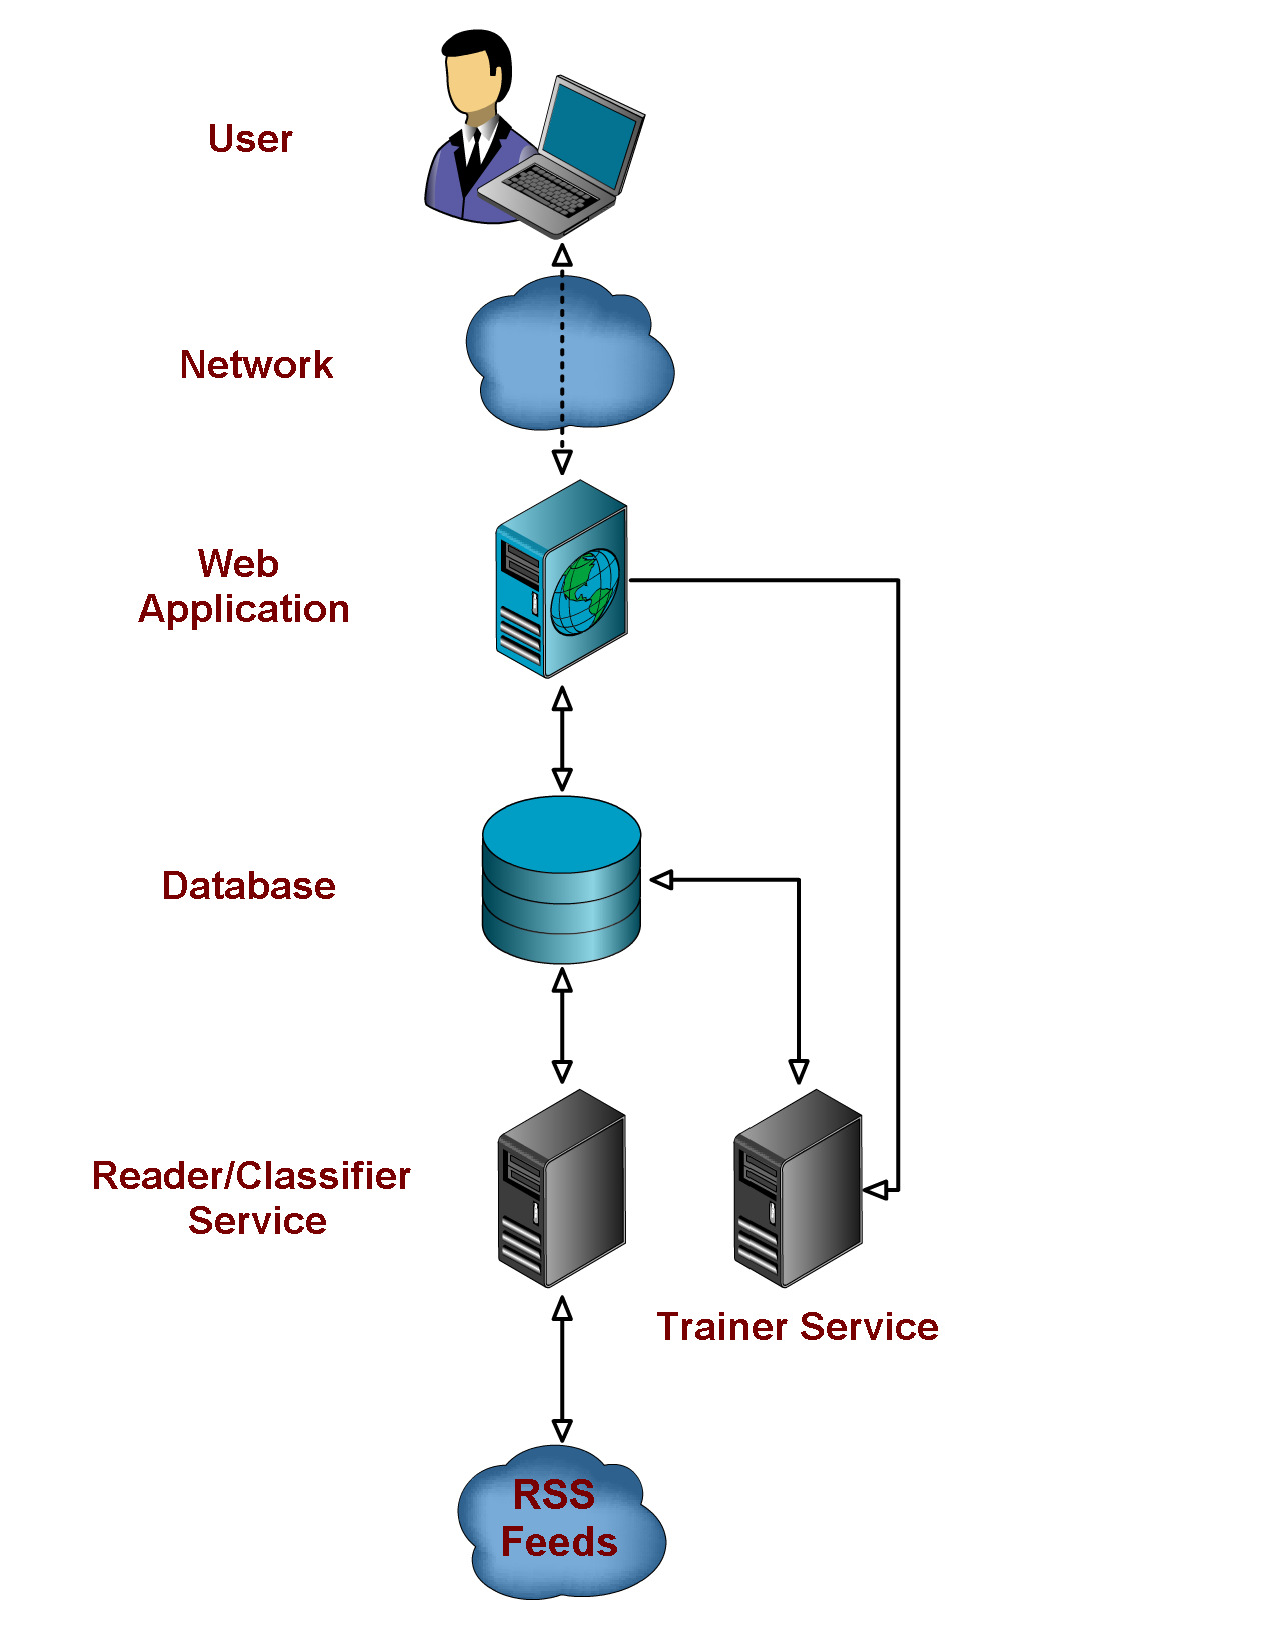
\includegraphics[width=4in]{arch-diagram.pdf}

The web application serves as the user interface, and displays/updates information on the database. Whenever a user gives input that serves as training data, the appropriate information is put on the database and a signal is sent to the trainer service telling it what to process.

The reader service checks RSS feeds at regular intervals, classifies their news items, and stores them to the database.

The trainer service listens for signals from the web application, and trains/updates database-stored classifier objects according to the indicated training data.

\subsection{Database}
//TODO: Insert database diagram

\section{Implementation}
\subsection{Web Interface}
The user interface is purely a web interface.  The implementation was created using Django, a Python web-framework.  When a user is created it, it has an initial special category, Trash. All documents that fail to be categorized properly end up in the Trash.  The user has the ability to create as many categories as he or she chooses.  These categories will remain empty unless the user adds feeds, which is where the news items will come from. Both of these can  As news-items are categorized, the user will see them appear

\subsection{Trainer Service}
The trainer service checks a message queue (see Message Queue subsection) to get training items (each of which consists of a classifier ID, a desired category ID, and a document's text).
Whenever a message or messages are available on the queue, A batch of training items of the same classifier ID are collected, which are put in a runnable job for execution by a threadpool.

If multiple batches have the same classifier ID (for example, if new items are added to the message queue when a thread is in the process of training), the access layer for the classifier/trainer objects ensures subsequent threads ones must wait for the preceeding thread to finish.

The actual training is done with \texttt{NaiveBayesTrainer} objects from the Mallet framework \cite{McCallumMALLET}.
Each training thread acquires a \texttt{NaiveBayesTrainer} object (either deserialized from database, or instantiated for initial training),
passes the training items through a custom filter such that they are converted to objects the Mallet framework is compatible with,
runs these instances through the \texttt{ClassifierTrainer},
and persists the trainer and classifier back to the database.

\subsection{Reader/Categorizer Service}
The reader service retreives a list of Feed urls from the database using a certain polling interval. Each time it does this, it creates and starts a series of threadpool jobs to retrieve the RSS data (using the Informa framework \cite{Informa}). When these jobs have all finished, the service creates another series of threadpool jobs, one for each news item. Each of these threads will retrieve the latest classifier for their associated user (deserialized from database), use it to determine the best category, and store their item to the database with the corresponding category ID.

The classifier object is a \texttt{NaiveBayes} classifier from the Mallet framework (trained by the trainer service). The classifier can return a vector of category/probability pairs. The thread doing the classifying will determine the most probable category, and confirm that its probability scaled by the number of categories is at least greater than some value, and categorizes it as trash otherwise. (The rationale for this being that if there are three categories where the most probable category has probability 0.34, and the others have probability 0.33, then this represents a very uncertain classification, and it would be better to put it in the trash as effectively uncategorized.)

\subsection{Message Queue}
\label{MessageQueueSection}
The trainer service uses a custom Message Queue module for receiving user feedback on classification.

The web application layer makes socket connections to a listening thread spawned by the trainer service.//TODO

\section{Analysis}
Quantitative analysis of the Mallet Framework's Naive Bayes classifier was done using data from Reuters-21578 corpus \cite{Reuters21578} (a collection of pre-categorized news articles made available for research purposes).

Since some of the news articles in this collection are listed under multiple categories, and our model allows one category per news item, we set up our parser to ignore all items that span multiple categories. Out of the 21578 articles, there are 9002 that have singular categories.

We created an analysis program to use a Mallet Naive Bayes classifier in the same manner in which it is used in the main project, train it using a variable portion of the data (randomly selected), and test it using the remaining portion.

We also set up a testing option where a number of categories are artifically grouped together as a ``trash'' category, to simulate typical use of our system.

For the number of non-trash categories being 66, 30, and 5, we ran with each of these $16\times 19=304$ trials, (16 trials for each of 19 different training ratios). Results are given below.

\subsection{Results}
Each marker represents the average accuracy of the 16 trials for the specified number of non-trash categories and number of training items.

The error bars signify the maximum and minimum accuracies found over the 16 trials.\\

\noindent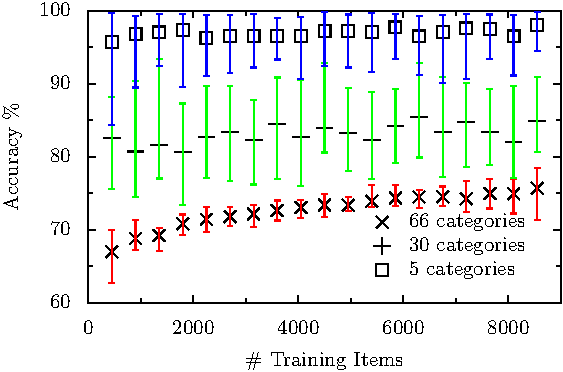
\includegraphics[width=3.35in]{data.pdf}

\subsection{Conclusion}
From the analysis,//TODO

\bibliography{bibliography}
\bibliographystyle{aaai}
\end{document}
